% !TEX root = ../Presentation.tex
% ---------------------------------------------------------------------------
% Plan of the talk and the terms used for the data
% ---------------------------------------------------------------------------
\section{Terms}

\begin{frame}{Today}
  \Large
  \begin{enumerate}
    \item The terms I use for the data
    \item Three models of the data
    \item What they show
    \item Open questions for you
  \end{enumerate}
\end{frame}

\begin{frame}{Two kinds of trial}
  \centering
  \begin{tikzpicture}[scale=0.8, every node/.append style={transform shape=false}]
    \trialpanel{0}{0}
    \draw[muted!60, line width=0.8pt] (4.75,-0.8) -- (4.75,5.9);
    \trialpanel{6.6}{1}
  \end{tikzpicture}
  \par\vspace{0.4em}
  \textbf{Group:} hand $\times$ trial type, so four groups: left/right, unimanual/bimanual
\end{frame}

\begin{frame}{Each session has one distractor amplitude}
  \centering
  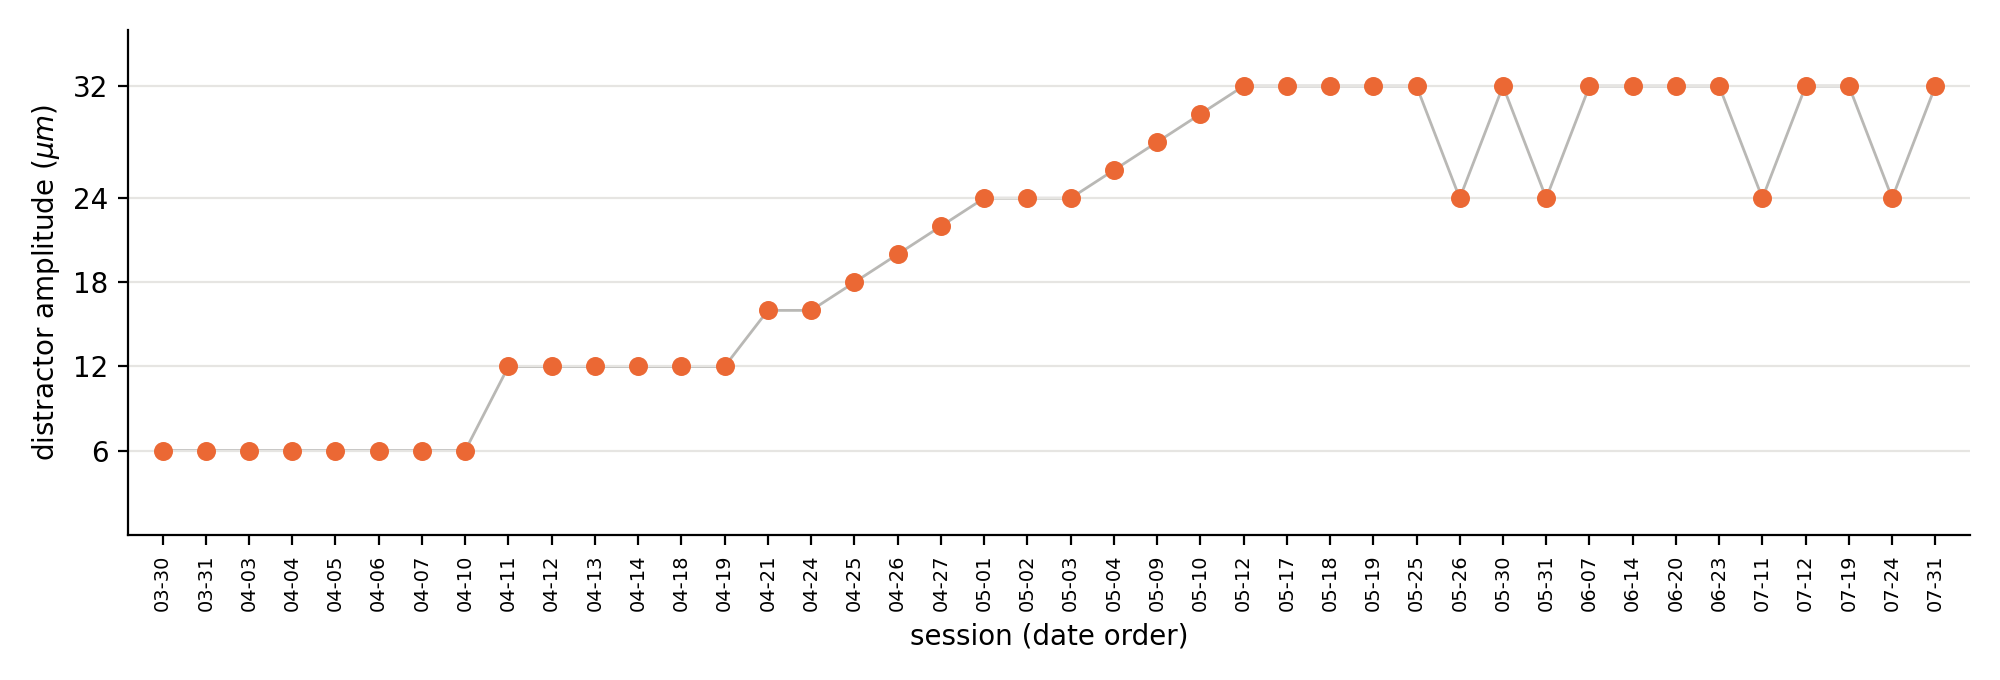
\includegraphics[width=\textwidth]{amplitude_schedule.png}
  \par\vspace{0.3em}
  42 sessions of about 300 trials, from one monkey (Sirius)
\end{frame}

\begin{frame}{The psychometric curve}
  \begin{columns}[c]
    \begin{column}{0.52\textwidth}
      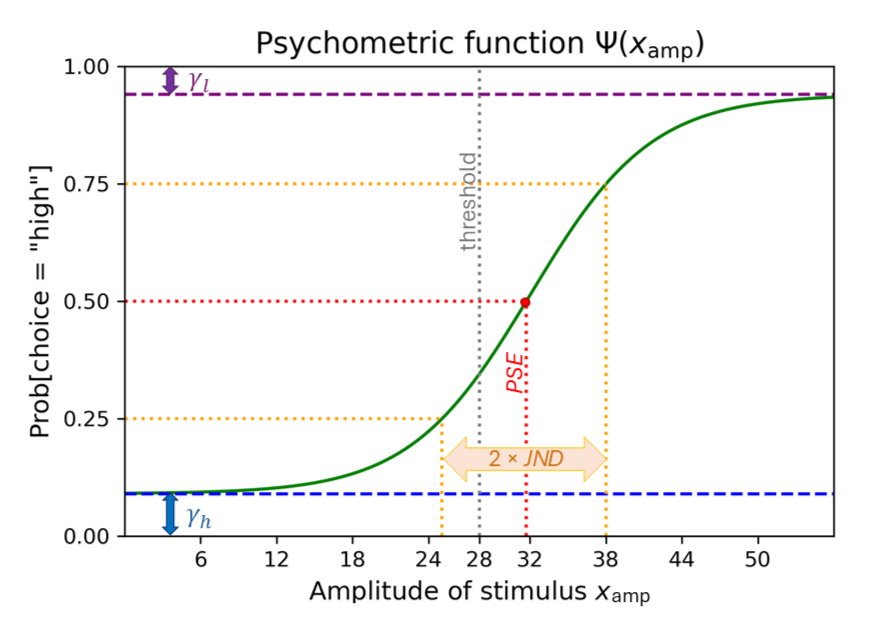
\includegraphics[width=\textwidth]{../Presentation_ABC/example_psych_func.png}
    \end{column}
    \begin{column}{0.46\textwidth}
      \small
      \begin{itemize}
        \setlength{\itemsep}{0.5em}
        \item \textbf{PSE} (bias): called ``high'' half the time\\
              {\color{muted}lower PSE = more ``high'' answers}
        \item \textbf{JND} (sensitivity): how fast the curve rises\\
              {\color{muted}larger JND = less precise}
        \item \textbf{Lapses:} answers the stimulus does not explain\\
              {\color{muted}${\color{blue}\gamma_h}$ = floor, ${\color{purple}\gamma_l}$ = gap below the ceiling}
      \end{itemize}
    \end{column}
  \end{columns}
  \vspace{0.5em}
  \centering
  \textbf{Distractor effect} = bimanual $-$ unimanual, for each hand
\end{frame}
